% !TEX encoding = UTF-8 Unicode
\documentclass[a4paper]{article}

\usepackage{color}
\usepackage{url}
\usepackage[T2A]{fontenc} % enable Cyrillic fonts
\usepackage[utf8]{inputenc} % make weird characters work
\usepackage{graphicx}
\usepackage{multirow}

\usepackage[english,serbian]{babel}
%\usepackage[english,serbianc]{babel} %ukljuciti babel sa ovim opcijama, umesto gornjim, ukoliko se koristi cirilica

\usepackage[unicode]{hyperref}
\hypersetup{colorlinks,citecolor=green,filecolor=green,linkcolor=blue,urlcolor=blue}

\usepackage{listings}

\newcommand\todos[1]{\textcolor{red}{#1}}

%\newtheorem{primer}{Пример}[section] %ćirilični primer
\newtheorem{primer}{Primer}[section]

\definecolor{mygreen}{rgb}{0,0.6,0}
\definecolor{mygray}{rgb}{0.5,0.5,0.5}
\definecolor{mymauve}{rgb}{0.58,0,0.82}

\lstset{ 
  backgroundcolor=\color{white},   % choose the background color; you must add \usepackage{color} or \usepackage{xcolor}; should come as last argument
  basicstyle=\footnotesize,        % the size of the fonts that are used for the code
  breakatwhitespace=false,         % sets if automatic breaks should only happen at whitespace
  breaklines=true,                 % sets automatic line breaking
  captionpos=b,                    % sets the caption-position to bottom
  commentstyle=\color{mygreen},    % comment style
  deletekeywords={...},            % if you want to delete keywords from the given language
  escapeinside={\%*}{*)},          % if you want to add LaTeX within your code
  extendedchars=true,              % lets you use non-ASCII characters; for 8-bits encodings only, does not work with UTF-8
  firstnumber=1000,                % start line enumeration with line 1000
  frame=single,	                   % adds a frame around the code
  keepspaces=true,                 % keeps spaces in text, useful for keeping indentation of code (possibly needs columns=flexible)
  keywordstyle=\color{blue},       % keyword style
  language=Python,                 % the language of the code
  morekeywords={*,...},            % if you want to add more keywords to the set
  numbers=left,                    % where to put the line-numbers; possible values are (none, left, right)
  numbersep=5pt,                   % how far the line-numbers are from the code
  numberstyle=\tiny\color{mygray}, % the style that is used for the line-numbers
  rulecolor=\color{black},         % if not set, the frame-color may be changed on line-breaks within not-black text (e.g. comments (green here))
  showspaces=false,                % show spaces everywhere adding particular underscores; it overrides 'showstringspaces'
  showstringspaces=false,          % underline spaces within strings only
  showtabs=false,                  % show tabs within strings adding particular underscores
  stepnumber=2,                    % the step between two line-numbers. If it's 1, each line will be numbered
  stringstyle=\color{mymauve},     % string literal style
  tabsize=2,	                   % sets default tabsize to 2 spaces
  title=\lstname                   % show the filename of files included with \lstinputlisting; also try caption instead of title
}

\begin{document}

\title{Programski jezik SWIFT\\ \small{Seminarski rad u okviru kursa\\Metodologija stručnog i naučnog rada\\ Matematički fakultet}}

\author{Anđelković Dragica, Nikolić Igor, Pejović Petar, Mandić Igor\\ andjelkovic.dragica96@gmail.com, igor.nikolic032@hotmail.com,\\ petar.pejovic8@gmail.com, igormandic996@gmail.com}

%\date{9.~april 2015.}

\maketitle

\abstract{
U ovom tekstu je ukratko prikazana osnovna forma seminarskog rada.}


\tableofcontents

\newpage

\section{Uvod}
\label{sec:uvod}
Swift je novi programski jezik  opšte namene razvijen od strane kompanije Apple za iOS, macOS, watchOS, tvOS, Linux i z/OS. Dizajniran je da radi u Apple radnim okruženjima, Cocoa i Cocoa Touch i  postojećeg Objective-C koda pisanog za Apple proizvode. Podržava imperativni, objektno-orjantisani i funkcionalni način programiranja. Napravljen je upotrebom LLVM programskog prevodioca otvorenog koda i ukljucen je u Xcode, počev od verzije 6. Swift koristi izvršno okruženje programskog jezika Objective-C, što omogućava izvršavanje C, C++, Objective-C i Swift koda u okviru jednog programa.
Namera kompanije Apple je bila  da Swift podrži mnoge ključne koncepte povezane sa programskim jezikom Objective-C.




\section{Nastanak i istorijski razvoj}
\label{sec:prviDeo}

Razvoj programskog jezika Swift je započeo 2010. godine Chris Lattner, koji je implementirao veći deo osnovne strukture jezika, za čije je postojanje znala samo nekolicina ljudi. Tek su krajem 2011. godine i drugi programeri počeli da sarađuju na projektu Swift, a u julu 2013 godine on je posato glavni fokus grupe Apple Developer Tools.

Swift je predstavljen na međunarodnoj konferenciji programera (WWDC - Worldwide Developers Conference) 2014. godine, uz integrisano razvojno okruženje Xcode 6 i OS 8. U decembru 2015. godine Apple je zvanično izdao Swift kao projekat otvorenog koda i pokrenuo je veb sajt \url{http://swift.org}, koji je posvećen zajednici Swift. Swift skladište se nalazi na GitHub stranici kompanije Apple (\url{http://github.com/apple}). Swift razvojno skladište (\url{https://github.com/apple/swift-evolution}) prati napredak Swifta, dokumentujući predložene promene. U razvojnom skladištu se može pronaći lista predloženih promena koje su prihvaćene i onih koje su odbijene. Swift 3 sadrži nekoliko poboljšanja koje je preporučila zajednica programera. U tabeli \ref{tab:tabela1} se nalaze sve do sada izbačene verzije programskog jezika Swift, u hronološkom redosledu.

\begin{table}[h!]
\begin{center}
\caption{Istorijski razvoj programskog jezika Swift.}
\begin{tabular}{|c|c|} \hline
\label{tab:tabela1}
Datum & Verzija \\ \hline
2014-09-09 & Swift 1.0 \\ \hline
2014-10-22 & Swift 1.1 \\ \hline
2015-04-08 & Swift 1.2 \\ \hline
2015-09-21 & Swift 2.0 \\ \hline
2016-09-13 & Swift 3.0 \\ \hline
2017-09-19 & Swift 4.0 \\ \hline
2018-03-29 & Swift 4.1 \\ \hline
2018-09-17 & Swift 4.2 \\ \hline
2019-02-28 & Swift 4.3 \\ \hline
2019-03-25 & Swift 5.0 \\ \hline
\end{tabular}
\end{center}
\end{table}



Prvu verziju karakteriše REPL alat koji omogućava izvršavanje  manjih fragmenata Swift koda i njegovo testiranje sa komandne linije. Swift 1.1 je samo mali iskorak, rešeni su manji propusti i rađeno je na stabilnosti. U Swift 1.2 verziji uvedena je nova struktura podataka - skup. Ova verzija je donela poboljšanja performansi kompajlera i smanjila vreme potrebno za kompajliranje Swift programa. Prilikom pokretanja projekta, kompajliraju se samo fajlovi kod kojih je detektovana izmena, što je posebno značajno kod većih projekata. Unapređeno if-let vezivanje tako da je moguće proveriti više uslova u jednom redu.


U drugoj verziji, kao deo novog projekta, predstvljen je Swift paket menadžer za upravljanje Swift bibliotekama. Kao priprema za naredne verzije dodata je provera verzije izvršnog okruženja. Glavne funkcionalnosti koje su ugrađene u programski jezik u drugoj verziji su:
\begin{itemize}
\item programiranje orjentisano na protokole,
\item model za obradu grešaka,
\item odlaganje izvršavanja naredbe pomoću ključne reči defer,
\item provera da li je funkcija dostupna na trenutnoj verziji uređaja i platforme koja pokreće našu aplikaciju pomoću ključne reči available.
\item vezivanje opcionih  vrednosti pomoću iskaza guard. 
\end{itemize}



Treća verzija sadrži osnovne promene u samom jeziku i biiblioteci Swift standarda, zbog toga nije kompatibilan sa prethodnim verzijama Swift jezika. Jedan od osnovnih ciljeva autora Swifta 3 je da on bude kompatibilan na više platformi, tako da kod koji se napiše za jednu platformu bude kompatibilan na svim drugim platformama. To znači da će kod koji se napise za MAC OS funkcionisati i na Linuxu. Tranzicija od Swift 2 je bila veoma velika I tezka programerima za ispravljanje, projekti su prijavljivali gomilu gresaka koji su bile teske za ispravljanje tako da su mnogi projekti pocinjani ispocetka



Četvrta verzija je kompatibilna sa trećom. Nove karakteristike koje je podržala četvrta verzija su:
\begin{itemize}
\item parsiranje fajlova u json i xml formatu,
\item jednostrano definisani opsezi,
\item poboljšanje funkcionalnosti struktura podataka: rečnik i skup,
\item kombinovanje klasa i protokola,
\item pisanje generičkih podskripti.
\item Velike promene  u string API-u
\end{itemize}


Dodata su sledeća poboljšanja u petoj verziji:
\begin{itemize}
\item karakteri u stringu imaju dodatne property-e
\item metoda za ostatak pri deljenju koja vraća bool
\item Unapređen rad sa vise rečnika.
\item Dodat je novi tip result 
\item ABI stability – rad u različitim verzijama jezika istovremeno
\end{itemize}
  
\subsection{Mesto u razvojnom stablu i uticaji drugih programskih jezika}
\label{subsec:podnaslov6}
Na razvoj Swifta uticali su mnogi programski jezici, od kojih su najznačajniji: Objective-C, Ruby, Haskell, C\#, Python. Preuzeti su određeni delovi iz različitih programskih jezika i poboljšani. Pregled preuzetih koncepata se nalaze u tabeli \ref{tab:tabela2}.

\begin{table}[h!]
\begin{center}
\caption{Preuzeti koncepti iz drugih programskih jezika.}
\begin{tabular}{|c|c|} \hline
\label{tab:tabela2}
Programski jezik & Šta je preuzeto \\ \hline
JavaScript & Rečnik (heš mape) \\ \hline
Scala i Opa & Zaključivanje tipova \\ \hline
Cold Fusion i JSP & Interpolacija Stringa \\ \hline
Python & Opciono naznačavanje kraja naredbe \\ \hline
Java i C\# & Protokoli (Interfejsi) \\ \hline
Lisp i Python & Tuples \\ \hline
Lisp i JavaScript &  Closure funkcije \\ \hline
C\# i Objective-C & Signed i unsigned int. \\ \hline
\end{tabular}
\end{center}
\end{table}
\section{Osnovna namena, svrha i mogućnosti}	
\label{sec:drugiDeo}


Pomoću Swift programskog jezika moguće je razviti bilo koji tip iOS i macOS aplikacija. Cilj Swift projekta je da stvori najbolji raspoloživi jezik za upotrebu od programiranja sistema, preko razvoja mobilnih i desktop aplikacija do cloud usluga. Takođe, ubrzan je proces razvoja proizvoda, poboljšane su performanse i povećana sigurnost aplikacija.

Jedna od glavnih namena Swift programskog jezika je kreiranje mobilnih aplikacija za iPhone i iPad uređaje. Swift je moguće izvršavati na Linux operativnom sistemu i Raspberry Pi. Članovi zajednice rade na stvaranju Swift aplikacija koje će se izvršavati i na Android platformama.

Osim što je Swift poznat po razvoju aplikacija za Apple platforme, koristi se i u modernim server aplikacijama. Swift je odličan izbor za server aplikacije koje zahtevaju visoke performanse kompajlera, nizak stepen korišćenja memorije i visok nivo bezbednosti.

Swift je sve popularniji programski jezik za razvoj IoT aplikacija. Kako bi kompanija Apple postala lider u primeni IoT aplikacija, razvijene su biblioteke i razvojni okviri koje rade najveći deo posla, dok se programeri mogu fokusirati na funcionalnosti IoT aplikacija.

Neka od mogućnosti koje pruža pomoću svojih funkcija:
\begin{itemize}
\item Automatsko utvrđivanje tipova - Swift može automatski da utvrdi tip promenljive ili konstante na osnovu inicijalne
vrednosti. 
\item Generički tipovi - generički tipovi omogućavaju da se piše kod jednom za izvršenje identičnih
zadataka za različite tipove objekata dok se zadržava bezbednost tipa. 
\item Promenljivost kolekcije - Swift nema posebne objekte za promenljive ili nepromenljive kontejnere. Umesto
toga, možete da definišete promenljivost definisanjem kontejnera kao konstante
ili kao promenljive.
\item Sintaksa zatvorenog izraza - zatvoreni izrazi su samostalni blokovi funkcionalnosti koji mogu da se proslede i upotrebe u kodu.
\item Pseudoklase - pseudoklasa definiše promenljivu koja možda nema vrednost.
\item Switch iskaz - Switch iskaz je drastično poboljšan funkcijama, kao što su poklapanje šablona i
zaštitni uslovi; zahvaljujući njima, izbegnute su automatske greške.
\item Višestruki povratni tipovi - funkcije mogu da imaju višestruke povratne tipove upotrebom torki. 
\item Preklapanje operatora - klase mogu da obezbede sopstvenu implementaciju postojećih operatora. 
\item Nabrajanja sa pratećim vrednostima - u Swiftu može da se uradi mnogo više od jednostavnog definisanja grupe srodnih vrednosti pomoću nabrajanja.
\end{itemize}

Postoji još jedna funkcija, koja tehnički nije
funkcija Swifta, već Xcodea i kompajlera. To je Mix and match. Ona omogućava kreiranje aplikacija koje sadrže Objective-C i Swift fajlove. To omogućava da se sistematski ažuriraju aktuelne Objective-C aplikacije pomoću Swift klasa i upotrebu Objective-C biblioteka/radnih okvira u Swift aplikacijama.



\section{Osnovne osobine programskog jezika}	
\label{sec:treciDeo}

Swift je objektno orijentisan programski jezik, koji je Apple razvio sa ciljem da 
se poboljšaju određeni delovi jezika Objective-C, ali da se i iskoriste njegove
dobre osobine. Pored Objective-C, u jezik Swift su uključene i osobine i mnogih drugih jezika,
kao sto su Python, Java, Ruby, Haskell. Najvažnije osobine programskog jezika Swift su:
\begin{itemize}
\item\textbf{Objektno orijentisan} - moderan objektno orijentisan jezik.
\item\textbf{Funkcionalan} - sadrži osobine zbog kojih je pogodan za pisanje funkcionalnih programa.
\item\textbf{Jasan} - lako se čita i lako piše, ima minimalne sintaksne ukrase i samo nekoliko skrivenih prečica. Njegova sintaksa je jasna, dosledna i očigledna.
\item\textbf{Bezbedan} - zahteva jake tipove kako bi obezbedio da u svakom trenutku i on i programer znaju na šta se sve tipovi objekata pozivaju.
\item\textbf{Ekonomičan} - mali jezik koji nudi samo neke osnovne tipove podataka i funkcionalnosti. Preostalo mora da bude dato kodom programera ili bibliotekama(razvojno okruženje Cocoa).
\item\textbf{Upravlja memorijom} - automatski upravlja memorijom i programer ne treba o tome da brine.
\item\textbf{Kompatibilnost sa razvojnim okruženjem Cocoa}
\end{itemize}

Ove osobine čine Swift izuzetnim jezikom za učenje iOS programiranja.


\subsection{Veza sa Objective-C}
\label{subsec:podnaslovVeza}

Jezik Swift predstavlja unapređenu, intuintivniju i pregledniju verziju jezika Objective-C.
Nedostaci programskog jezika Objective-C u odnosu na Swift su:
\begin{itemize}
\item Delimično objektno orijentisan - Objective-C objektno orijentisane osobine je preuzeo od 		      jezika C. Sadrži i objekte i skalarne tipove podataka, sa tim što se objekti 
	  nalaze unutar posebnog C tipa podataka(pokazivača).
\item Sintaksa može da bude složena i teska za razumevanje.
\item Provera tipova često može da se isključi, i često je isključena.
\item Koristi ručno upravljanje memorijom.
\end{itemize}

Glavna osobina jezika Objective-C je kompatibilnost sa razvojnim okruženjem Cocoa.
Cocoa API interfejsi su ugrađene komande, sa kojima kod programera mora da sarađuje kako bi
se bilo šta dogodilo na nekom iOS uređaju. Cocoa Api interfejs je napisan u jezicima Objective-C i C. Swift je napravljen tako da može koristi većinu API interfejsa razvojnog okruženja Cocoa, i
to mu omogućava pisanje iOS aplikacija. 





\subsection{Podržane paradigme}
\label{subsec:podnaslovParadigma}

Programski jezik Swift je objektno orijentisani jezik, ali podržava i funkcionalno i imperativno
programiranje. Sadrži sve osnovne koncepte objektno orijentisanog programiranja, i objektno orijentisana paradigma je najzastupljenija u ovom jeziku. Međutim, nekoliko osobina Swift jezika, kao što su funkcije prvog reda, sofisticirani sistem tipizacije, lambda izrazi, korišćenje Karijevih funkcija i parcijalna aplikacija, čine jezik posebno pogodnim za pisanje funkcionalnih programa. Swift, kao funkcionalni jezik, može se u svakodnevnoj praksi koristiti za pisanje kraćih, elegantnijih i sigurnijih programa, koji su lakši za održavanje, nadgradnju i testiranje.




\section{Okruženja i njihove karakteristike}	
\label{sec:cetvrtiDeo}

Programski jezik Swift se može pisati u različitim okruženjima. Najpoznatije okruženje je \textbf{XCode}, a pored njega, koriste se i AppCode, Atom, CLion,SublimeText.

\subsection{XCode}
\label{subsec:podnaslovXCode}



XCode je integrisano razvojno okruženje koje je napravila kompanija Apple. Koristi se za razvoj iOS i macOS aplikacija. U ovom okruženju mogu se pisati kodovi u mnogim programskim jezicima, kao sto su C, C++, Objective-C, Java, AppleScript, Python, Ruby i Swift. XCode sadrži i okvire, i za programski jezik Swift su najvažniji \textbf{Playground} i \textbf{Cocoa Touch}. 
Postoji 9 verzija ovog okruženja, a od 6, obuhvata i programski jezik Swift.
\vspace{5mm}


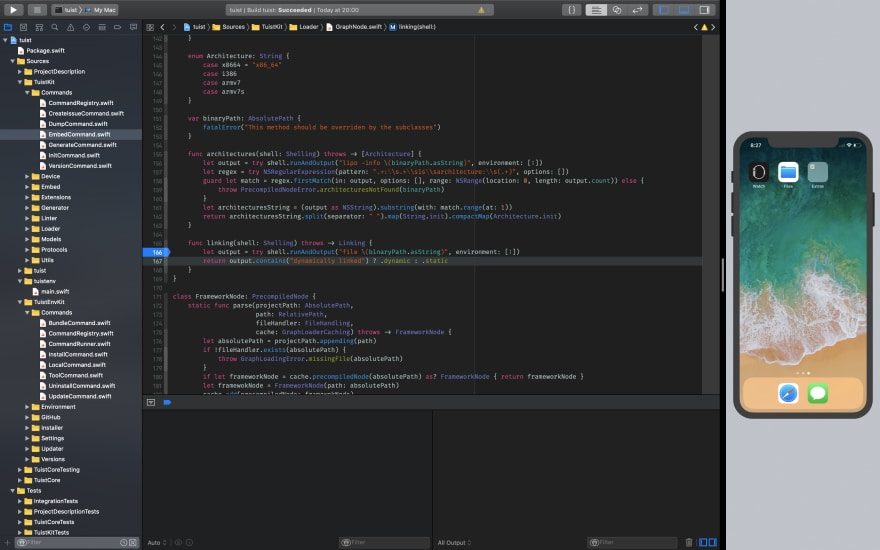
\includegraphics[scale=0.2]{xcode.jpg}


\subsection{Playground}
\label{subsec:podnaslovPlayground}
\vspace{5mm}


Playground je interaktivno radno okruženje koje omogućava da pišemo kod i odmah vidimo
rezultate čim su promene izvršene u kodu. Kako bi mogli da koristimo ovaj okvir potrebno je prvo
da pokrenemo Xcode i zatim izaberemo opciju Get started with a playground.
Sastoji se od nekoliko delova, među kojima su najvažniji: 
\begin{itemize}
\item prostor za kodiranje
\item bočna traka za rezultate
\item prostor za ispravljanje gresaka
\end{itemize}
\vspace{5mm}


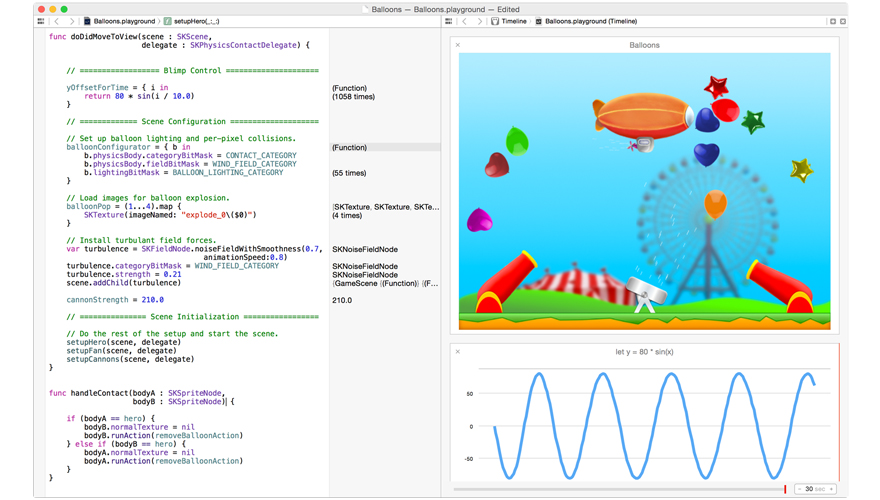
\includegraphics[scale=0.2]{playground.jpg}

\subsection{SublimeText}
\label{subsec:podnaslovSublimeText}

\vspace{5mm}




Sublime Text je verovatno jedan od najrasprostranjenijih okruzenja. Poseduje dobar korisnicki interfejs i sjajne performanse. On u osnovni podrzava mnoge programske jezike a nove funkcionalnosti mogu biti dodate koriscenjem dodataka(plugina), koji je zajednica razvijala pod licencom slobodnog softvera. Vrlo lako ga mozemo prilagoditi za razvoj swift aplikacija dodatkom podrske za swift pakete.
\vspace{5mm}


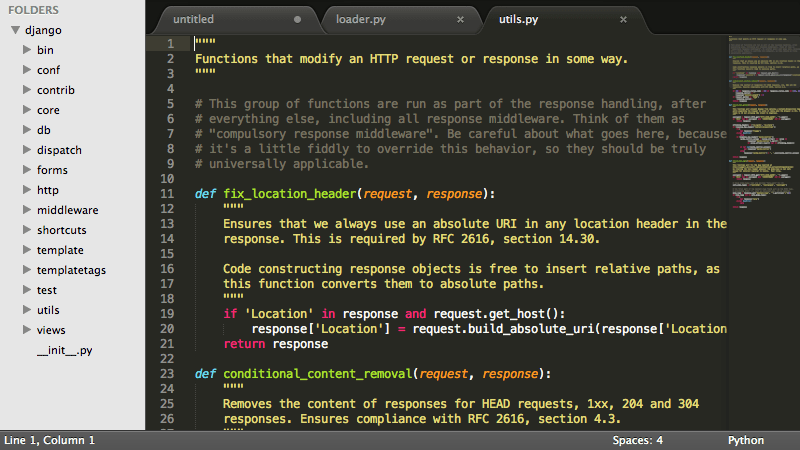
\includegraphics[scale=0.3]{sublime.png}

\subsection{Atom}
\label{subsec:podnaslovAtom}
\vspace{5mm}
Razvijen je od strane GitHub-a, visoko modularno okruzenje koje omogucava laku instalaciju novih paketa sto ga je svrstalo medju najpozeljnija okruzenja. Dodavanje podrske za swift programiranje je jednostavno instaliranjem language-swift paketa.

\vspace{5mm}

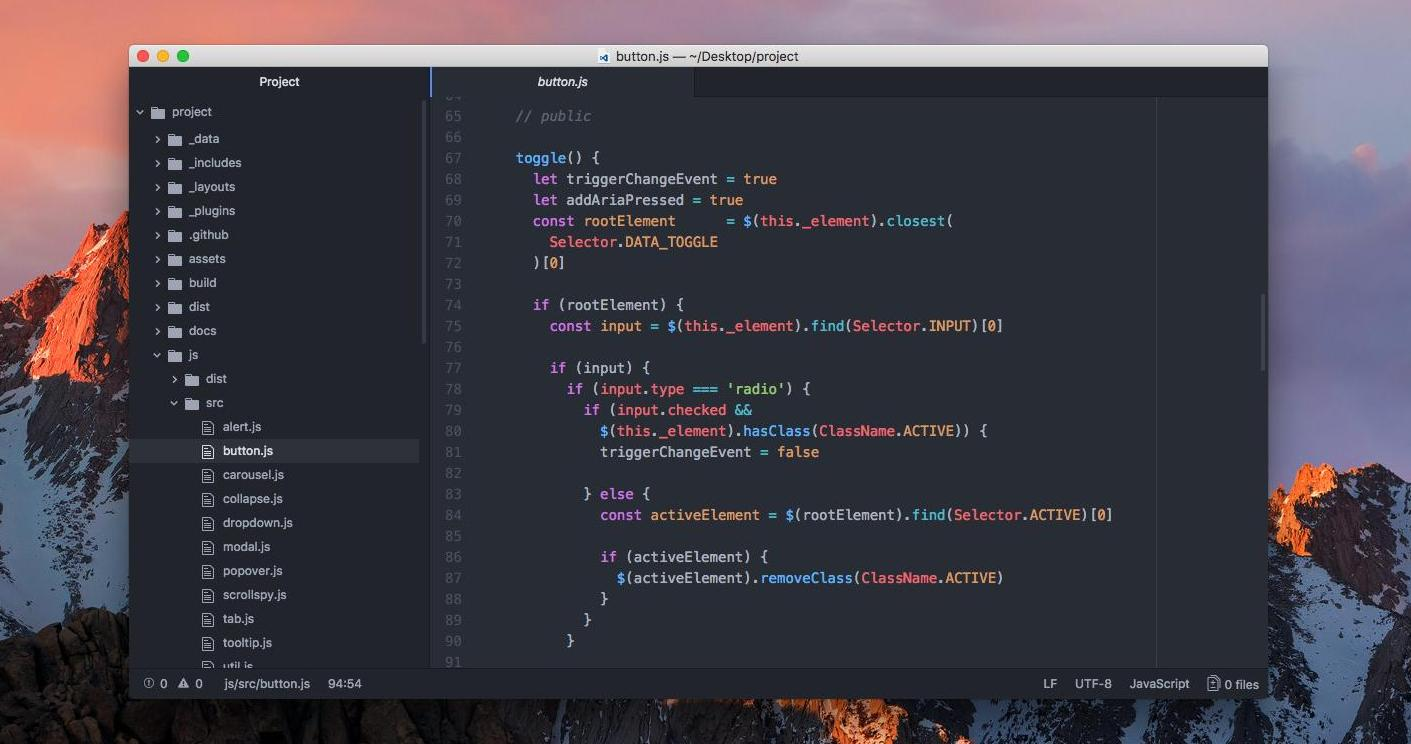
\includegraphics[scale=0.2]{atom.jpg}
\vspace{20mm}

\section{Instalacija i uputstvo za pokretanje}	
\label{sec:petiDeo}

\subsection{SWIFT na Windowsu}
\label{subsec:podnaslovWindows}

Na pocetku bice nam potreban editor teksta u kome zelimo da kodiramo. Mozemo koristiti bilo koje od gore navedenih razvojnih okruzenja u kojim nam je udobno da radimo. 
U ovom primeru koristicemo \href{https://notepad-plus-plus.org/download/v7.6.4.html}{Notepad++}, koji je jednostavan,besplatan i lak za instalaciju.
\vspace{5mm}

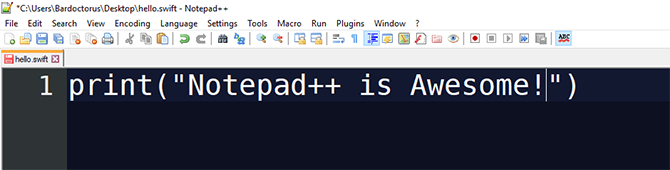
\includegraphics[scale=0.5]{notepadpp.png}
\vspace{5mm}

Nakon instaliranja napisacemo jednostavan program koji cemo kasnije pokrenuti pomocu Windows komandne linije. Prvo je potrebno da otvorimo novi Notepad++ fajl i u njega unesemo komandu za ispis.

\begin{lstlisting}[caption={},frame=single, label=simple]

print("Hello world!")



\end{lstlisting}
\vspace{5mm}
Da bi sacuvali ovaj kod,koristicemo File > Save As i izabrati Swift file iz Save As Type menija.Ako u meniju nedostaje tip ovog fajla izabracemo all files, i dodati .swift fajl ekstenziju nakon sto smo izabrali odgovarajuce ime.


\subsection{Kompiliranje}
\label{subsec:podnaslovKompiliranje}

Sada kada imamo program,zelimo da ga kompiliramo i pokrenemo. Kako ne postoji kompajler za swift koji je integrisan u Windowsu moramo da instaliramo. Han Sangjin je napravio kompajler za Swift koji je moguce skinuti sa Github-a. Nakon sto preuzmemo i instalirmo Swift za Windows aplikacije korisnicki interfejs bi trebao da izgleda ovako:

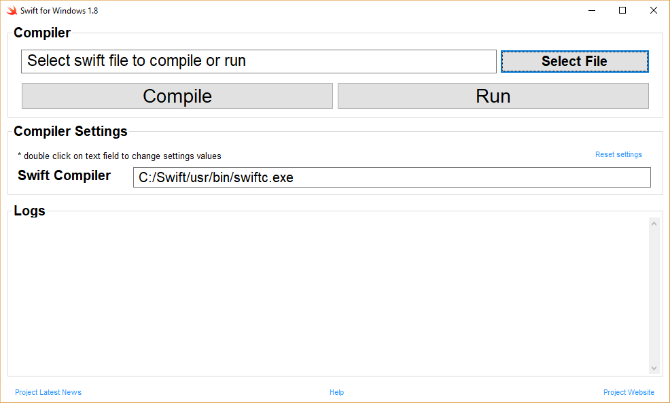
\includegraphics[scale=0.4]{swift-win.png}
\vspace{5mm}


Nakon pritiska na Select File izabracemo nas program koji smo prethodno napisali i pritisnuti Compile. Nakon sto sacekamo da se kompilacije zavrsi dobicemo poruku “Successfully compiled”.
Jednom kompiliran program mozemo pokrenuti neograniceni broj puta.



\subsection{SWIFT na Linuxu}
\label{subsec:podnaslovLinux}

Kao i u prethodnom primeru bice nam potreban tekst editor gde cemo napisati jednostavan kod.
Mozemo koristiti bilo koji integrisani editor koji linux poseduje. Na isti nacin cemo iskodirati poruku za ispis "Hello World" kao u prethodnom primeru. I sacuvacemo nas program sa ekstenzijom .swift.

Da bismo koristili SWIFT na linuxu moramo ga prvo instalirati.U terminalu kucamo sledece komande:


\begin{lstlisting}[language=bash]

	wget https://swift.org/builds/ubuntu1510/swift-2.2-SNAPSHOT-2015-12-10-a/swift-2.2-SNAPSHOT-2015-12-10-a-ubuntu15.10.tar.gz

\end{lstlisting}
Nakon preuzimanja,pozicioniracemo se u folder Downloads i tamo raspakovati arhivu u kojoj se nalazi swift instalacija.



\begin{lstlisting}[language=bash]
  cd ~/Downloads
  tar -xvzf swift-2.2-SNAPSHOT*
\end{lstlisting}

Kada raspakujemo fajl potrebno je podesiti putanja do BIN-a kako bi mogli da izvrsavamo programe.

\vspace{5mm}

\begin{lstlisting}[language=bash]
  cd ~/Downloads/swift-2.2-SNAPSHOT*
  cd usr/bin
  pwd
\end{lstlisting}

Kao rezultat komande pwd dobicete tacnu lokaciju koju cemo koristiti.Kopirajte je i zamenite je na sledeci nacin.
\begin{lstlisting}[language=bash]
  export PATH=path_to_swift_usr_bin:$PATH

\end{lstlisting}
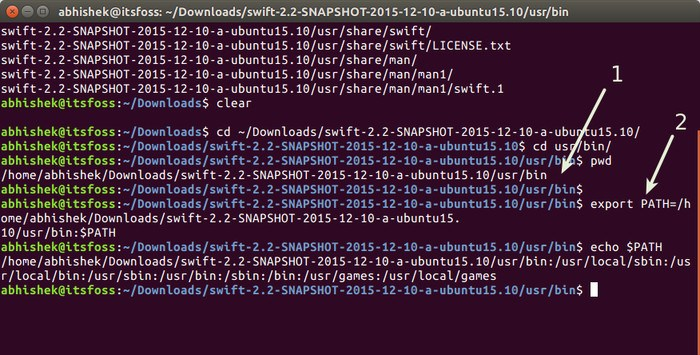
\includegraphics[scale=0.4]{swift-lin.jpeg}


Zatim moramo instalirati jos par biblioteka kako bi omogucili da swift nesmetano funkcionise na linuxu.


\begin{lstlisting}[language=bash]
  sudo apt-get install clang libicu-dev
  swift -version
\end{lstlisting}

I na kraju da bismo kompilirali i pokrenuli prethodno napisan program potrebno je da ukucamo sledece komande:

\begin{lstlisting}[language=bash]
  swift imeprograma.swift
  ./imeprograma
\end{lstlisting}



\section{Primer jednostavnog koda i njegovo objašnjene}	
\label{sec:sestiDeo}

U narednim primerima biće prikazane i objašnjene osnovne funkcionalnosti jezika Swift.

\begin{lstlisting}[caption={},frame=single, label=simple]

print("Hello world!")
print("Hello world!");

\end{lstlisting}

Ispis teksta se vrši pomoću funkcije print(). Tačka-zarez su opcioni na kraju svakog reda.\\



\begin{lstlisting}[caption={},frame=single, label=simple]

var x = 5
var y = 3

if x == 5 {
	print("x je 5");
}

if (x==3) {
	print("x je 5");
}

if (x == 5)				//Syntax error
	print("x je 5");

\end{lstlisting}

Nije strogo tipiziran (deklarišemo promenljive pomocu - var), a dodeljujemo vrednost pomoću operatora dodele.\\
Zagrade kod provere uslova su opcione. Preporučujemo da se zagrade ne koriste, osim u slučaju kada imate više uslovnih iskaza u istoj liniji.\\
Velike (vitičaste) zagrade moraju se koristiti kod if-grane i petlji, u suprotnom će doći do greške.\\
I za uslovne iskaze (if i while) i za iskaze dodele (=) razmaci su opcioni.\\



\begin{lstlisting}[caption={},frame=single, label=simple]

var ime = "Swift"
var jezik = "programski jezik"

var poruka = " je najbolji "
var poruka1 = "\ (ime) je najbolji \ (jezik) !" 

print(ime,poruka,jezik,"!")
print(poruka1)

\end{lstlisting}

Stringovi se takodje dodeljuju pomoću operatora dodele.\\
Konkatenacija stringova se vrši pomoću specijalnih karaktera '$\backslash$ (string)' ili jednostavnim navodjenjem u naredbi 'print', gde se stringovi razdvajaju zarezima.\\



\begin{lstlisting}[caption={},frame=single, label=simple]

var ime1 = "Swift"
var ime2 = "Java"
var ime3 = "Python"
var ime3 = ""

print(ime1,ime2,ime3,separator:", ", terminator:"")
print(ime1,ime2,ime3,separator:", ", terminator:"", to:&ime4)

\end{lstlisting}

Listu stringova koji su razdvojeni određenim separatorom, pravimo pomoću naredbe print, gde se prvo navode stringovi koji čine tu listu, a nakon toga separator i terminator.\\
Možemo koristiti jos jedan parametar u funkciji print(), pod nazivom toStream. Pomoću njega preusmeravamo ispis funkcije print(). Konkretno u ovom primeru preusmeravamo ispis u promenljivu ime4.\\


\begin{lstlisting}[caption={},frame=single, label=simple]

var x:Int = 0
for x in 0...10 {
	print(x)
}

var y:String = ""
while y != "aaaaa" {
	print(y)
	y = y + "a"
}

\end{lstlisting}

U ovom primeru je pokazana funkcionalnost for i while petlje. Takodje jos jednom i mogućnost konkatenacije pomoću operatora +. Nakon for petlje u konzoli će biti ispisani brojevi od 0 do 10. U while petlji će se svakog puta dodavati po jedno slovo a, i tako 5 puta.


\begin{lstlisting}[caption={},frame=single, label=simple]

var score:Int = 0
var currency:Float = 0

func addToScore(points:Int, money:Float){
	score = score + points
	currency = currency + money
}

addToScore(points: 30, money: 1.45)
addToScore(points: 60, money: 2.86)

print(score)
print(currency)

\end{lstlisting}

Pozivanje funkcije sa parametrima koja nema povratnu vrednost. Nakon dva poziva, u kojima moramo proslediti dva argumenta funcije, bice ispisana dva broja (90-score i 4.31-currency).\\


\begin{lstlisting}[caption={},frame=single, label=simple]

var x:Int = 1

func function() -> Bool {
	if(x == 0){
		return false
	} else {
		return true
	}
}

var y:Bool = function()

\end{lstlisting}

Pozivanje funkcije koja ima povratnu vrednost. Nakon poziva povratna vrednost funkcije u ovom slučaju je true, koju ujedno dobija i promenljiva y.\\






\section{Specifičnosti}	
\label{sec:sedmiDeo}


Moj deo \\
Moj deo \\
Moj deo \\
Moj deo \\




\section{Zaključak}
\label{sec:zakljucak}

Ovde pišem zaključak. 
Ovde pišem zaključak. 
Ovde pišem zaključak. 
Ovde pišem zaključak. 
Ovde pišem zaključak. 
Ovde pišem zaključak. 
Ovde pišem zaključak. 
Ovde pišem zaključak. 
Ovde pišem zaključak. 
Ovde pišem zaključak. 
Ovde pišem zaključak. 
Ovde pišem zaključak. 


\addcontentsline{toc}{section}{Literatura}
\appendix
\bibliography{seminarski} 
\bibliographystyle{plain}

\appendix

\end{document}
\grid
\grid
